% !TeX root = ../document.tex

\section{Interpolation methods}

The following chapter describes interpolation in general with regard to the most frequently used methods. We will give an introduction to the background of each method, their suitability/advantages and disadvantages as well as examples of application in other studies. Furthermore, we present possibilities of carrying out interpolation analysis and an overview of which methods are supported by a variety of FOSSGIS tools.


\subsection{Statistical and Deterministic methods?}

A deterministic method always generates the exact same output for a given input. Thus, leading to reproducible results, whereas a statistical method might not generate the same results.
% TODO: Should we keep this?

\subsection{What is spatial interpolation?}

Spatial interpolation is the calculation of nearby and unknown values ​​on the basis of neighboring known values. \cite{gitta_raumliche_2016} Interpolation methods are often used for analyzing spatial and spatio-temporal distributions of physical but also socioeconomic phenomena. These phenomena can be approximated by certain functions, which are location dependent within space \cite{mitas_spatial_1999}. Interpolation is thus very useful for estimating or predicting missing geographic point data, such as elevation, rainfall, chemical concentrations, noise levels etc. \cite{samanta_interpolation_2012}. Calculating these unknown values is done via a series of different methods, where the methods themselves again depend on the research question and the data present. In this study we will be focusing on temperature data only and give a short overview of similar studies and their choice of method.

\subsection{The diversity of methods}

In this chapter, we will give a short introduction to the various methods, starting off with a general possibility of classification – a schematic overview. According to \citeauthor{hofstra_comparison_2008} the choice of method, when interpolating climate-related data, depends primarily on the different variables, station densities and climate regimes. It is rather difficult to find a single method which fulfills all requirements. Thus, the goal is to give an overview of different (and widely used) interpolation methods (mostly in the context of climate-related research) and present some advantages and disadvantages of each method as well as give some examples of their application.

\subsection{Schematic overview}

Generally, there is a difference between global and local interpolation, whereas global interpolation is not suitable for determining values ​​that are as exact as possible, but for assessing rough global spatial structures. \cite{gitta_raumliche_2016}
Interpolation methods are also distinguishable in exact and non-exact or gradual and abrupt interpolation (see figure \ref{fig:exact_non_exact_interploation}). On the left, the generated surface, which stands for the resulting interpolation, fits exactly to the data points, although the surface has abrupt  \ldq{}steps\rdq{} (the used method here is the Natural Neighbor interpolation). Adjusting the interpolation surface results in a smoother surface, as seen in figure \ref{fig:exact_non_exact_interploation} on the right.
% TODO: zweimal the used method...
The used method, the inverse distance weighting (IDW), does not follow the high and low data points exactly, which is why a \ldq{}moving average\rdq{} or \ldq{}smoothing\rdq{} of the data occurs. In the end, the choice depends on whether  \ldq{}[...] we need the interpolated surface to exactly pass through the data points or we require a surface which simply represents the general trend\rdq{}. \cite{wyatt_interpolation_nodate}



\begin{figure}
	\begin{minipage}[b]{.48\linewidth}
		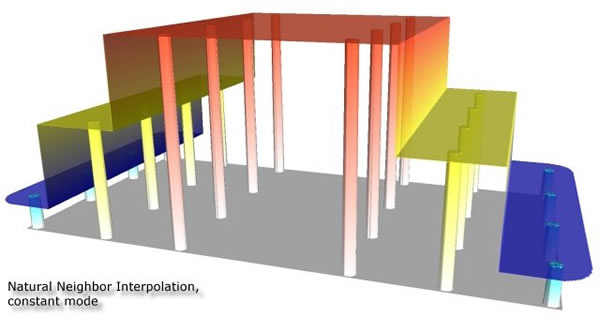
\includegraphics[width=\linewidth]{images/exakte_interpolation.jpg}
	\end{minipage}
	\hfill
	\begin{minipage}[b]{.48\linewidth}
		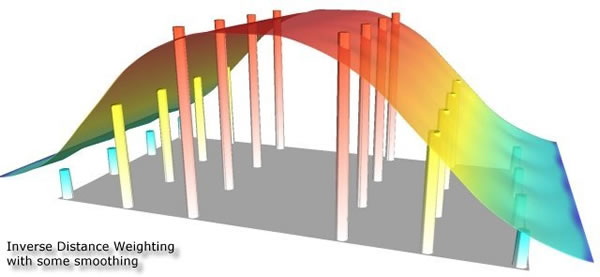
\includegraphics[width=\linewidth]{images/nicht_exakte_interpolation.jpg}
	\end{minipage}
	\caption{Different interpolation surfaces due to exact (left) and non-exact (right) interpolation\cite{gitta_raumliche_2016}}
	\label{fig:exact_non_exact_interploation}
\end{figure}

And finally, we can differentiate between deterministic and stochastic methods.\cite{gitta_raumliche_2016}
Deterministic methods encompass for example \ldq{}TIN\rdq{}, \ldq{}IDW\rdq{} or \ldq{}Spline\rdq{}. \cite{wasser_going_2020} Deterministic interpolation techniques are generally based on precisely predictable (= deterministic) spatial relationships, whereas stochastic (also called probabilistic or geostatistical) methods, make use of underlying statistical properties of the point data. Latter requires advanced knowledge, which is why will focus primarily on deterministic methods. One of the most prominent and important stochastic methods is Kriging.

In regard to suitability, we refer to figure \ref{fig:interpolation_methods_strengths}, which gives a good overview for several of the methods and their advantages and disadvantages. As the choice of method is, as already stated, dependent on the question one poses and the data available, no general statement can be given.


\begin{figure}[b!]
	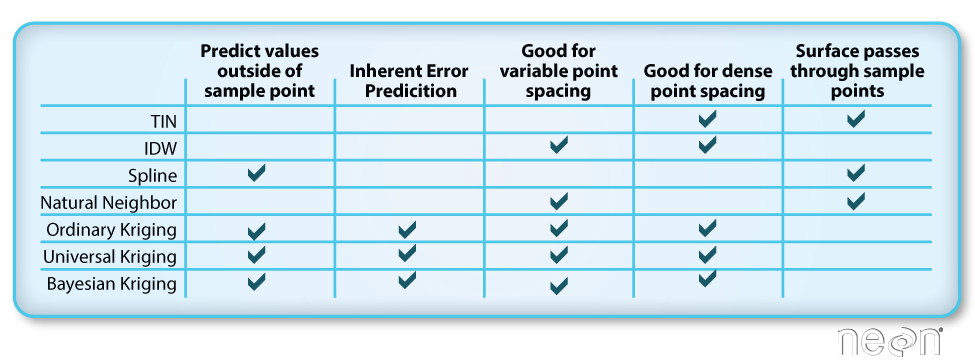
\includegraphics[width=\linewidth]{images/interpolation_methods_strengths.png}
	\caption{Strengths of interpolation methods \cite{wasser_going_2020}}
	\label{fig:interpolation_methods_strengths}
\end{figure}

\subsection{Common methods}

In a study by \citeauthor{wenjing_cao_study_2009}, the authors compared different interpolation methods for temperature values in China. Their results show that Kriging-exponential and Kriging-spherical methods are the best, or most accurate, interpolations methods, the interpolation precision of IDW is second, but, overall, Kriging-Gaussian and Spline interpolation methods have the lowest accuracy. \cite{wenjing_cao_study_2009} Other studies also show a similar application and result of comparing these methods: 
\citeauthor{hofstra_comparison_2008} compares the methods Natural Neighbour, Kriging and (thin plate) Splines. They conclude that global Kriging is best suitable for a daily climate data set (ibid.). Also \citeauthor{samanta_interpolation_2012} use the three common methods IDW, Kriging and Spline to estimate climate variables and temperature.
We have, therefore, decided to focus on the four methods: TIN, IDW, Kriging and Spline. We will present these methods shortly, give some examples of usage and their pros and cons.

\subsubsection{TIN}

TIN stands for \ldq{}Triangulated Irregular Network\rdq{}. Hereby, scattered points are linked into a set of triangles and the interpolation takes place directly along the edges of the triangle. The nearest neighbour is taken for each value to be interpolated. \cite{lam_spatial_2009} Points, which have more than a single neighbour form the network made of triangles. 
There are two main algorithms or geometric constructions to discern: Voronoi diagrams and Delaunay triangulations. \cite{sambridge_geophysical_1995} Without going into detail, Voronoi diagrams split up a plane based on a set of points (see figure \ref{fig:voronoi_delauny}(a)). Delauny triangulations, which are supported by the linear interpolation algorithm for the GDAL tool, form a surface of non-overlapping triangles (see figure \ref{fig:voronoi_delauny}(b)). For three points a circumference is formed. Thereby, three points form a valid triangle if there are no other points within the perimeter. If there are more than three points in the area, it is not defined which points are to be chosen.

\begin{figure}
	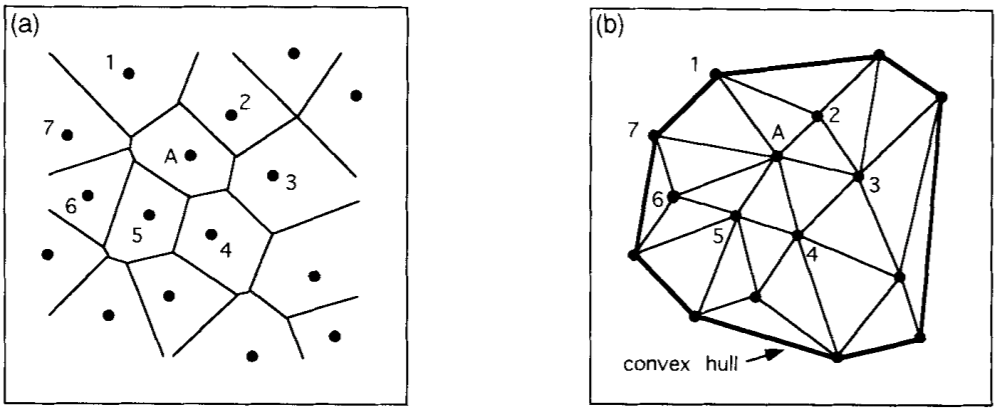
\includegraphics[width=\linewidth]{images/voronoi_delauny.png}
	\caption{(a) Voronoi diagram and corresponding (b) Delaunay triangulation\cite{sambridge_geophysical_1995}}
	\label{fig:voronoi_delauny}
\end{figure}

TIN is commonly used to produce contour maps and also shaded relief maps. \cite{lam_spatial_2009}
It should be noted that there are several ways of constructing the triangulation with the same set of points – thus, comparability is restricted. This method also results in sharp edges, and it is not recommended for analysis of the areas outside the selected data points. \cite{qgis_11_2021} Certainly, TIN is a popular method, which is available with most FOSSGIS tools. 

\subsubsection{Inverse Distance Weighting (IDW)}
IDW is a method whereby the distance between a predicted point and sample point is weighted. More precisely, \ldq{}[t]he sample points are weighted by the inverse of their distance to the predicted point\rdq{} \cite[p.2]{wenjing_cao_study_2009}, which simply means that more weight is given to nearby points than to points in the distance. \cite{lam_spatial_2009} This encompasses Tobler’s well-known assumption that \ldq{}[...] things that are close to one another are more alike than those that are farther apart\rdq{}. \cite{samanta_interpolation_2012}

The IDW method is not only very common, but easily implemented and rather flexible. It is also available for almost any FOSSGIS, but has some shortcomings. A disadvantage of the method is that it does not reproduce the local shape implied by data, but local extrema at the data points (see figure \ref{fig:dem_mitas}). \cite{mitas_spatial_1999} \citeauthor{lam_spatial_2009} points out that the method is, unfortunately quite easily affected by a possible uneven distribution of data points. Even if points are clustered, they will be assigned an equal weight (ibid.). Thus, if data points are following a certain trend, IDW will average it out. 
Overall, the IDW method allows for fast calculations, while different distances are integrated in the calculation and estimation of the missing values. \cite{gitta_raumliche_2016} The method is therefore useful for dense and equally distributed data points. \cite{wasser_going_2020} IDW is for example beneficial for phenomena such as noise, where the data distribution is correlated with distance. \cite{gis_resources_choosing_2013}

\begin{figure}
	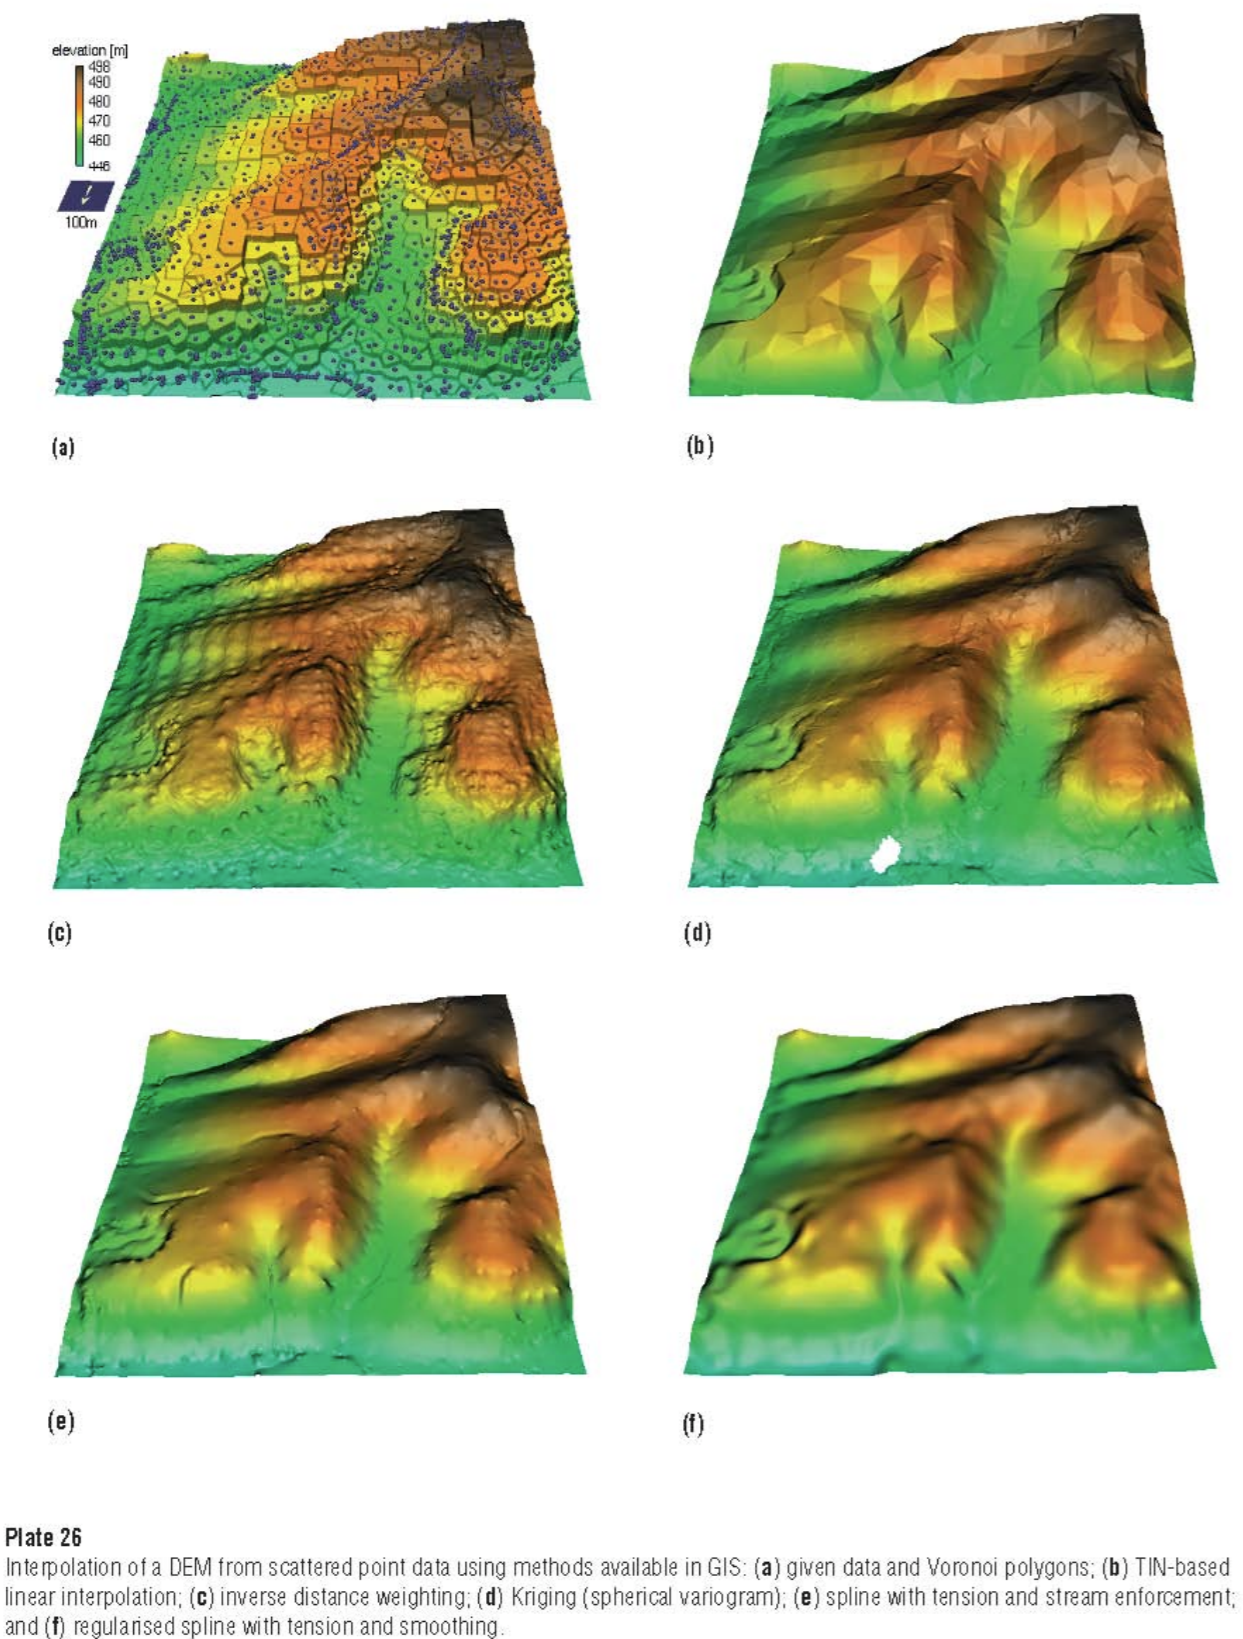
\includegraphics[width=\linewidth]{images/dem.png}
	\caption{Interpolation of a DEM and the result using (a) Voronoi polygons (b) TIN linear interpolation (c) IDW (d) Kriging and (e \& f) Spline (f includes smoothing) \cite{mitas_spatial_1999}}
	\label{fig:dem_mitas}
\end{figure}


\subsubsection{Kriging}

Kriging is a geostatistical approach with many variations. It is a complex interpolation, where it is assumed that \ldq{}[...] the distance or direction between sample points reflects a spatial correlation that can be used to explain variation in the surface\rdq{}. \cite[p.11605]{elumalai_spatial_2017} The method depends on weighting the measured points, the spatial relationships among the measured points around the predicted location, and the distance to the predicted location. \cite{wenjing_cao_study_2009}

Kriging, and other geostatistical approaches, have the capability of producing a prediction surface, and they can also provide some measure of certainty or accuracy of the predicted values. \cite{samanta_interpolation_2012} As (global) Kriging can exceed the known value range (not bound by minima and maxima), but does not pass through any of the sample points, the method is one of the best for all climate variables except maximum temperature. \cite{gis_resources_choosing_2013}

Even with a small number of sample points, Kriging will result in more accurate estimates than IDW. \cite{lam_spatial_2009} The advantage is that this method, as already mentioned is that it “[...] delivers a measure of confidence of how likely that prediction will be true” with an error estimation and a confidence interval for every unknown point. \cite{lam_spatial_2009} According to studies evaluated by \citeauthor{hofstra_comparison_2008}, (universal) kriging is best suitable for interpolating mean precipitation and temperature and daily climate variables. 

\subsubsection{Spline}

Spline is, as well as IDW, a deterministic method, which estimates missing values based on a mathematical function. The method minimizes overall \ldq{}surface curvature\rdq{} and results in a relatively smooth surface (compared to figure \ref{fig:dem_mitas}), passing exactly through the data points. \cite{samanta_interpolation_2012} That means a curved surface is adjusted to the sample points of the dataset. \ldq{}Imagine stretching a rubber sheet across your points and gluing it to each sample point along the way -- what you get is a smooth stretched sheet with bumps and valleys\rdq{} (as shown in figure \ref{fig:spline}). \cite{wasser_going_2020}

In comparison to TIN \& IDW, spline can also estimate data values outside the range of the given data points. Just like TIN, its surface will fit through the data points, unlike IDW or kriging methods (compare with figure \ref{fig:interpolation_methods_strengths}). In a dataset, where points are close together and have large value differences, spline is a disadvantage; especially for slope calculations as it can result in over- and underestimations. \cite{wasser_going_2020} Because spline interpolations smooths out abrupt or \ldq{}edgy\rdq{} changes in values, the method is not suitable, if these characteristics should remain preserved.

\begin{figure}
	\centering
	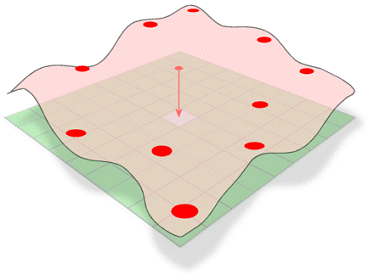
\includegraphics[width=.5\linewidth]{images/spline.png}
	\caption{Spline \ldq{}rubber sheet\rdq{} fit to known data points \cite{albrecht_spline_2005}}
	\label{fig:spline}
\end{figure}


\subsection{FOSSGIS Implementations}

\begin{table}[b!]
	\centering
	\begin{tabular}{c|c|c|c|c}
		Interpolation method & QGIS & GRASS GIS & SAGA & GDAL\\
		\hline
		Nearest neighbor & \xmark &\cmark &\cmark & \cmark \\
		\hline
		TIN & \cmark &\cmark &\cmark & \cmark \\
		\hline
		IDW & \cmark &\cmark &\cmark & \cmark \\
		\hline
		Spline & \xmark &\cmark &\cmark & \xmark \\
		\hline
		Kriging & \xmark &\cmark &\cmark & \xmark \\
	\end{tabular}
	\caption{\label{tab:table-name}Your caption.}
\end{table}







